% Chapter 4

\chapter{Benchmarking on Phantom datasets}
\label{chapter:benchmark}
\noindent\makebox[\linewidth]{\rule{0.75\paperwidth}{0.4pt}}
\noindent\makebox[\linewidth]{\rule{0.75\paperwidth}{0.4pt}}

\localtableofcontents % local toc

\noindent\makebox[\linewidth]{\rule{0.75\paperwidth}{0.4pt}}
\noindent\makebox[\linewidth]{\rule{0.75\paperwidth}{0.4pt}}
\newpage

\section{Introduction}
The last chapters define several ways to solve the inverse problem of MEG/EEG brain imaging techniques. The evaluation of these solvers remain difficult due to the completely unknown ground-truth of the exact localization of the involved sources in each specific task. This limitation is primarily coming from the fact that the recording is done over the scalp and that multiple source configurations can rise to exactly the same measurements over the sensors. So the question stayed unanswered of whether these long list of existing source localization techniques are able to locate the positions and the orientations with good precision giving appropriate cortex-based source models.

The way of this question is handled is typically by performing simulations. It consists on fixing the number and the location of several dipoles with some additive white Gaussian noise. These simulations are unfortunately rarely realistic, which do not take into account the non-ideal nature of the sensors, a realistic head geometries and the correlation with the noise. Furthermore, one needs to also consider the inaccuracies in the computation of the forward operator. There are mainly due to approximations in the conductivity values in the head and/or the numerical errors associated with either spherical head approximations or \ac{bem} based on more realistic head geometries. 

A more sophisticated simulations might be investigated to overcome these issues, but evaluation using data directly collected from an artificial physical object has the advantage that the results can more closely reflect \textit{in vivo} performance since they include factors that cannot readily be included in simulations, such as environmental noise and deviations of the physical system from our model. 

For this aim, artificial objects that mimic the brain activity called "\textit{phantoms}" are constructed by the manufacturers of MEG systems that we use to evaluate our solvers to the MEG/EEG inverse problem~\cite{hazim2015magnetoencephalography}. It is based on the theoretical description in~\cite{ilmoniemi1985forward} producing realistic data corresponding to complex spatio-temporal current sources including realistic head geometries. From 4 to 32 independent current dipoles were distributed with the "brain" region and MEG data was collected separately for each dipole. The true dipole locations and orientations and the morphology of the brain, skull layers were extracted from X-ray CT data~\cite{leahy1998study}. Its main limitation is that it is unsuitable for EEG.

This chapter presents a new study to validate dipole localization techniques using different exisiting phantom datasets. Other work has been done by~\cite{hazim2015magnetoencephalography,leahy1998study,baillet2001evaluation} using also real-skull phantom to investigate the performances of representative methods considering various head models.

The selected approaches are mainly those described here in this thesis, namely: Dipole fitting, Gamma-Map, RAP-MUSIC, MxNE, irMxNE, TF-MxNE, irTF-MxNE with and without multi-scale dictionary. The methods not defined so far, will be briefly described in the next section.

\section{Phantom datasets}
\subsection{Brainstorm phantom-elekta dataset}
The description was taken from the Brainstorm tutorial about the MEG phantom~\cite{tadel2011brainstorm}.\\

A current phantom is provided with Elekta Neuromag for checking the system performance and can be then used for evaluation of the source localization (Figure~\ref{fig:phantom_head}-Figure~\ref{fig:phantom_in_MEG}). It contains 32 artificial dipoles and four fixed head-position indicator coils. The phantom is based on the mathematical fact that an equilateral triangular line current produces equivalent magnetic field distribution to that of a tangential current dipole in a spherical conductor, provided that the vertex of the triangle and the origin of the conducting sphere coincide. For a detailed description of how the phantom works, see~\cite{ilmoniemi1985forward}.\\
\\

\begin{figure}[tb]
   \centering
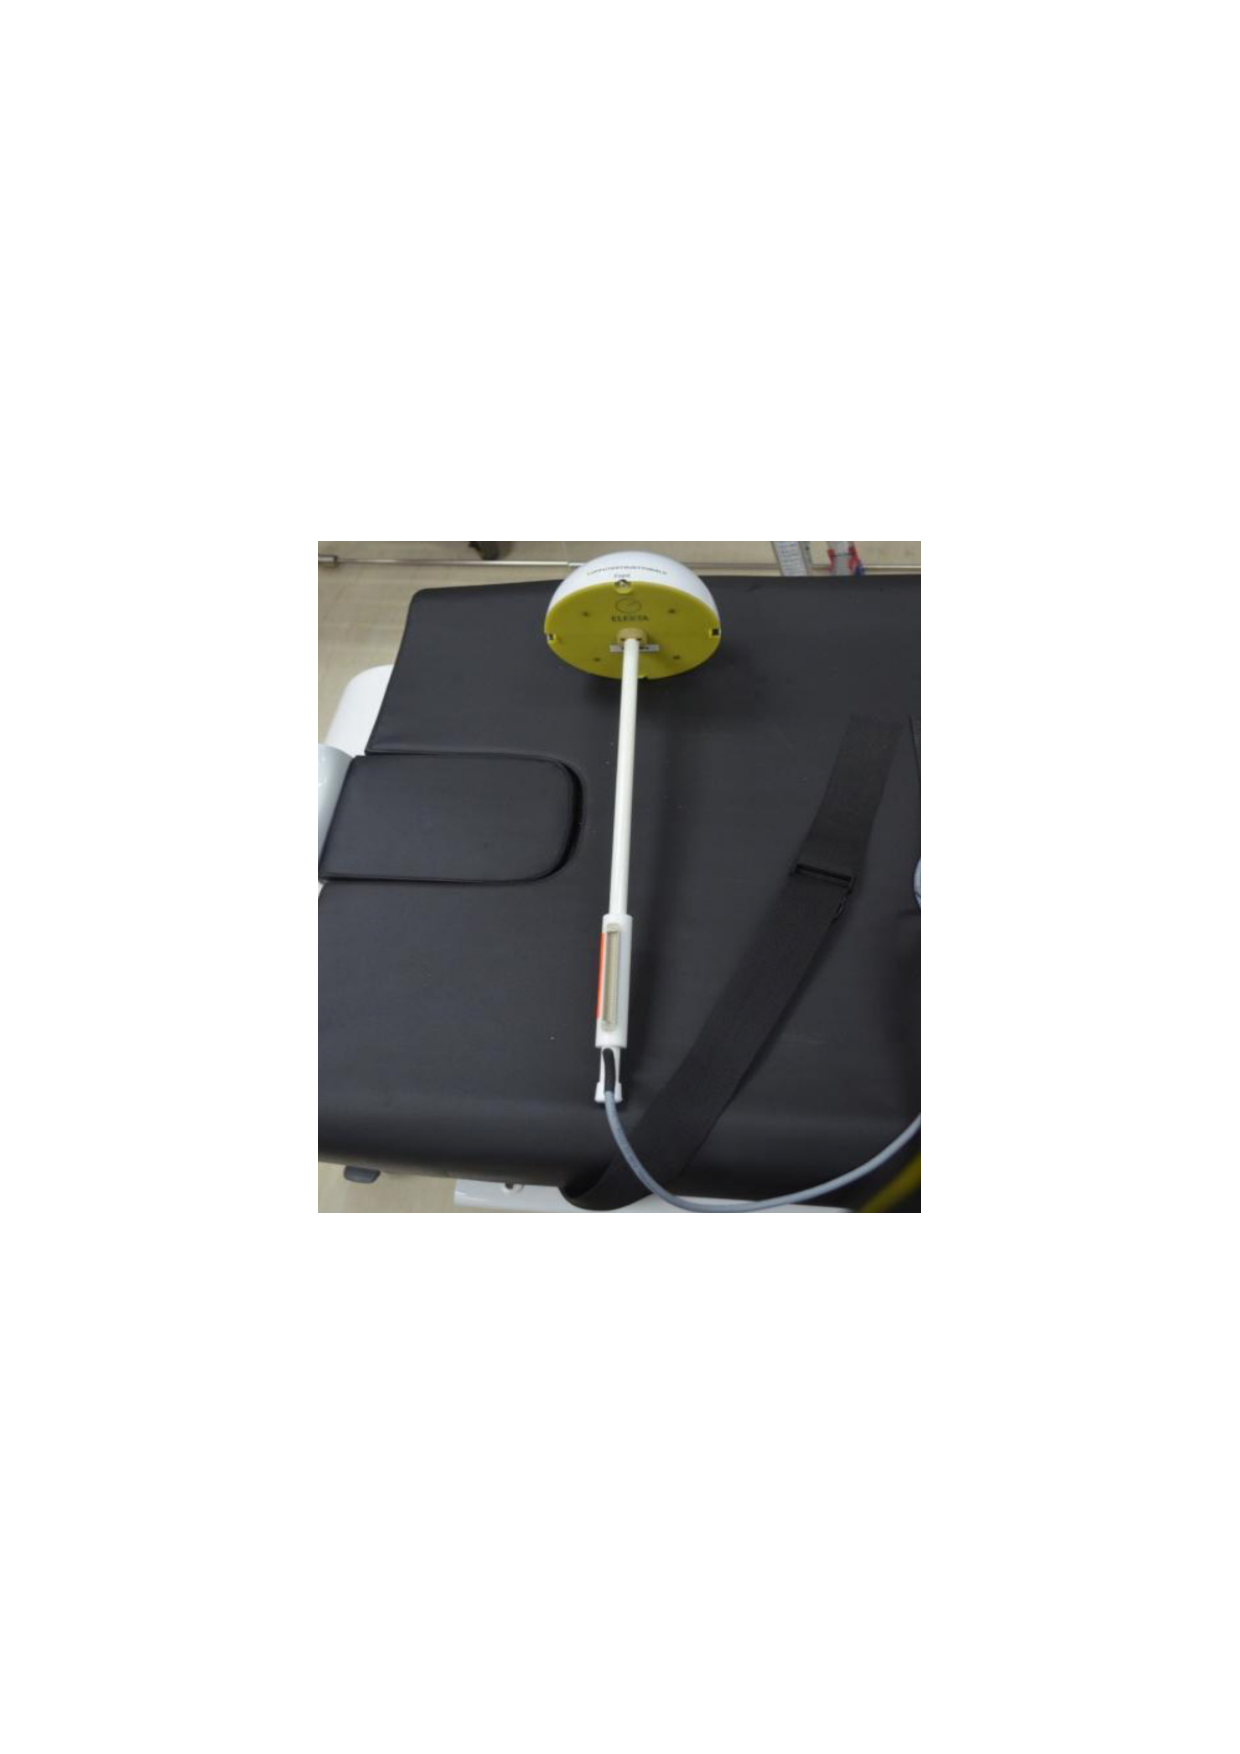
\includegraphics[trim={1cm 8cm 2cm 9cm},width = 0.97\textwidth]{benchmark/phantom_head}
\caption{Reference phantom (RefPhantom) NM24058N (Serial number: 101861) provided by Elekta Oy, Helsinki Finland. 32 built in simulated dipoles and four presetting head position indicator coils (HPI) (Figure taken from~\cite{hazim2015magnetoencephalography}).~\ref{alg:acceptreject}.}
   \label{fig:phantom_head}
\end{figure}

The phantom dipoles are energized using an internal signal generator which also feeds the HPI coils. An external multiplexer box is used to connect the signal to the individual dipoles. Only one dipole can be activated at a time. The location of the dipole is recorded relative to the center of the sphere (0,0,0)m, where X is positive toward the nasion, Y is positive toward the left ear and Z is positive toward the top of the head.\\

The dataset is sorted into four different SNR:
\begin{itemize}
\item Source with \textbf{2000 nAm}. This corresponds to an unrealistically strong 1000 nAm (2000 nAm peak-to-peak) dipole that gives the highest SNR of the experimental source.
\item Source with \textbf{200 nAm}. This is a weaker dipole, closer to the range of amplitudes we can expect in raw data.
\item Source with \textbf{20 nAm}. This represents some of the weakest sources we expect in evoked studies which require averaging to detect and estimate (\textit{i.e.} generally cannot be seen in single trial analysis).
\end{itemize}

\subsection{Brainstorm CTF-phantom dataset}

The dataset is sorted into four different SNR:
\begin{itemize}
\item Source with \textbf{200 nAm}. This is a weaker dipole, closer to the range of amplitudes we can expect in raw data.
\item Source with \textbf{20 nAm}. This represents some of the weakest sources we expect in evoked studies which require averaging to detect and estimate (\textit{i.e.} generally cannot be seen in single trial analysis).
\end{itemize}


\begin{figure}[tb]
   \centering
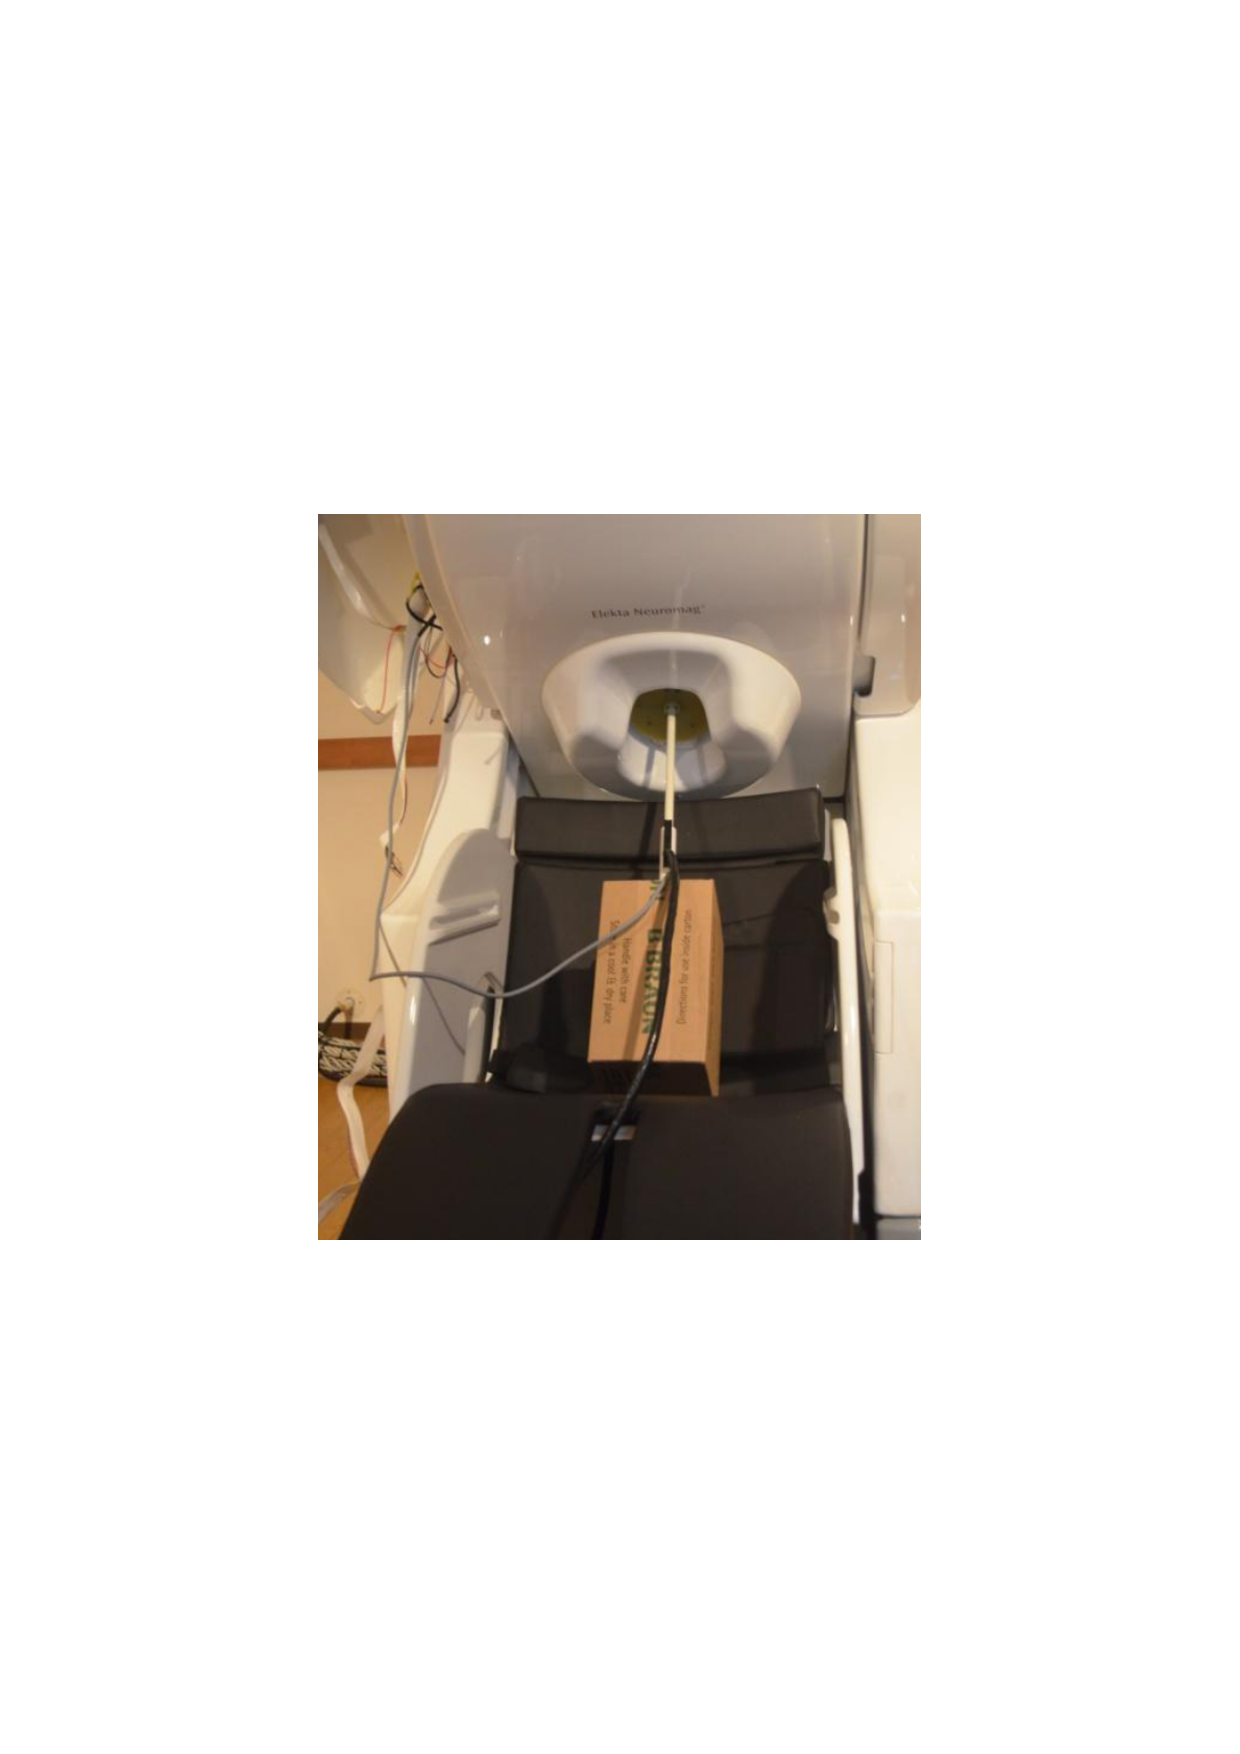
\includegraphics[trim={1cm 8cm 2cm 9cm},width = 0.97\textwidth]{benchmark/phantom_in_MEG}
\caption{Phantom is carefully set into sensor helmet of the probe unit and pushed again helmet. HPI coil is fitted into outlet under right gantry side cover (Figure taken from~\cite{hazim2015magnetoencephalography})~\ref{alg:acceptreject}.}
   \label{fig:phantom_in_MEG}
\end{figure}


\subsection{Brainstorm CTF-phantom dataset}

The dataset is sorted into four different SNR:
The dataset is sorted into four different SNR:
\begin{itemize}
\item Source with \textbf{2000 nAm}. This corresponds to an unrealistically strong 1000 nAm (2000 nAm peak-to-peak) dipole that gives the highest SNR of the experimental source.
\item Source with \textbf{200 nAm}. This is a weaker dipole, closer to the range of amplitudes we can expect in raw data.
\item Source with \textbf{100 nAm}. This is an even weaker dipole and a smaller SNR.
\item Source with \textbf{20 nAm}. This represents some of the weakest sources we expect in evoked studies which require averaging to detect and estimate (\textit{i.e.} generally cannot be seen in single trial analysis).
\end{itemize}

\section{Methodology}

\subsection{Sphere models}
The most commonly used head model assumes that it is made up of a set of nested concentric spheres, each with homogeneous and isotropic conductivity. Under this assumption, both the EEG and MEG problems admit to well known closed form solutions~\cite{mosher1999eeg}.

\subsection{The selected solvers}
\subsubsection{dipole fitting}
\subsubsection{Gamma Map}
\subsubsection{RAP MUSIC}
\subsubsection{MxNE}
\subsubsection{irMxNE}
\subsubsection{TF-MxNE}
\subsubsection{irTF-MxNE}

\section{Experimental results}

\subsection{Critical comparison of these MEG/EEG source localization}
\section{Discussion \& Conclusion}